\subsection{Questões \& Tarefas}

O processo de anotação semântica colaborativo é auxiliado por meio da definição de questões e tarefas. Quando um usuário possui algum dúvida específica em relação a anotação de um elemento de uma especificação WSDL, este usuário pode criar uma questão (\textit{issue}) associada ao elemento. Uma questão não é direcionada a um usuário específico, i.e., qualquer usuário envolvido na edição colaborativa é capaz de visualizar as questões para uma especificação WSDL e respondê-las. É possível ter múltiplas respostas de múltiplos usuários. Quando uma questão é considerada devidamente respondida, o usuário que a criou pode marcá-la como resolvida. A \figurename~\ref{fig:grasews-lista-issues} ilustra a interface gráfica de Grasews para a listagem de questões. Por meio desta interface gráfica, um usuário pode adicionar respostas às questões e marcá-las como resolvidas.

\begin{figure}[h]
    %\resizebox{\textwidth}{!}{
        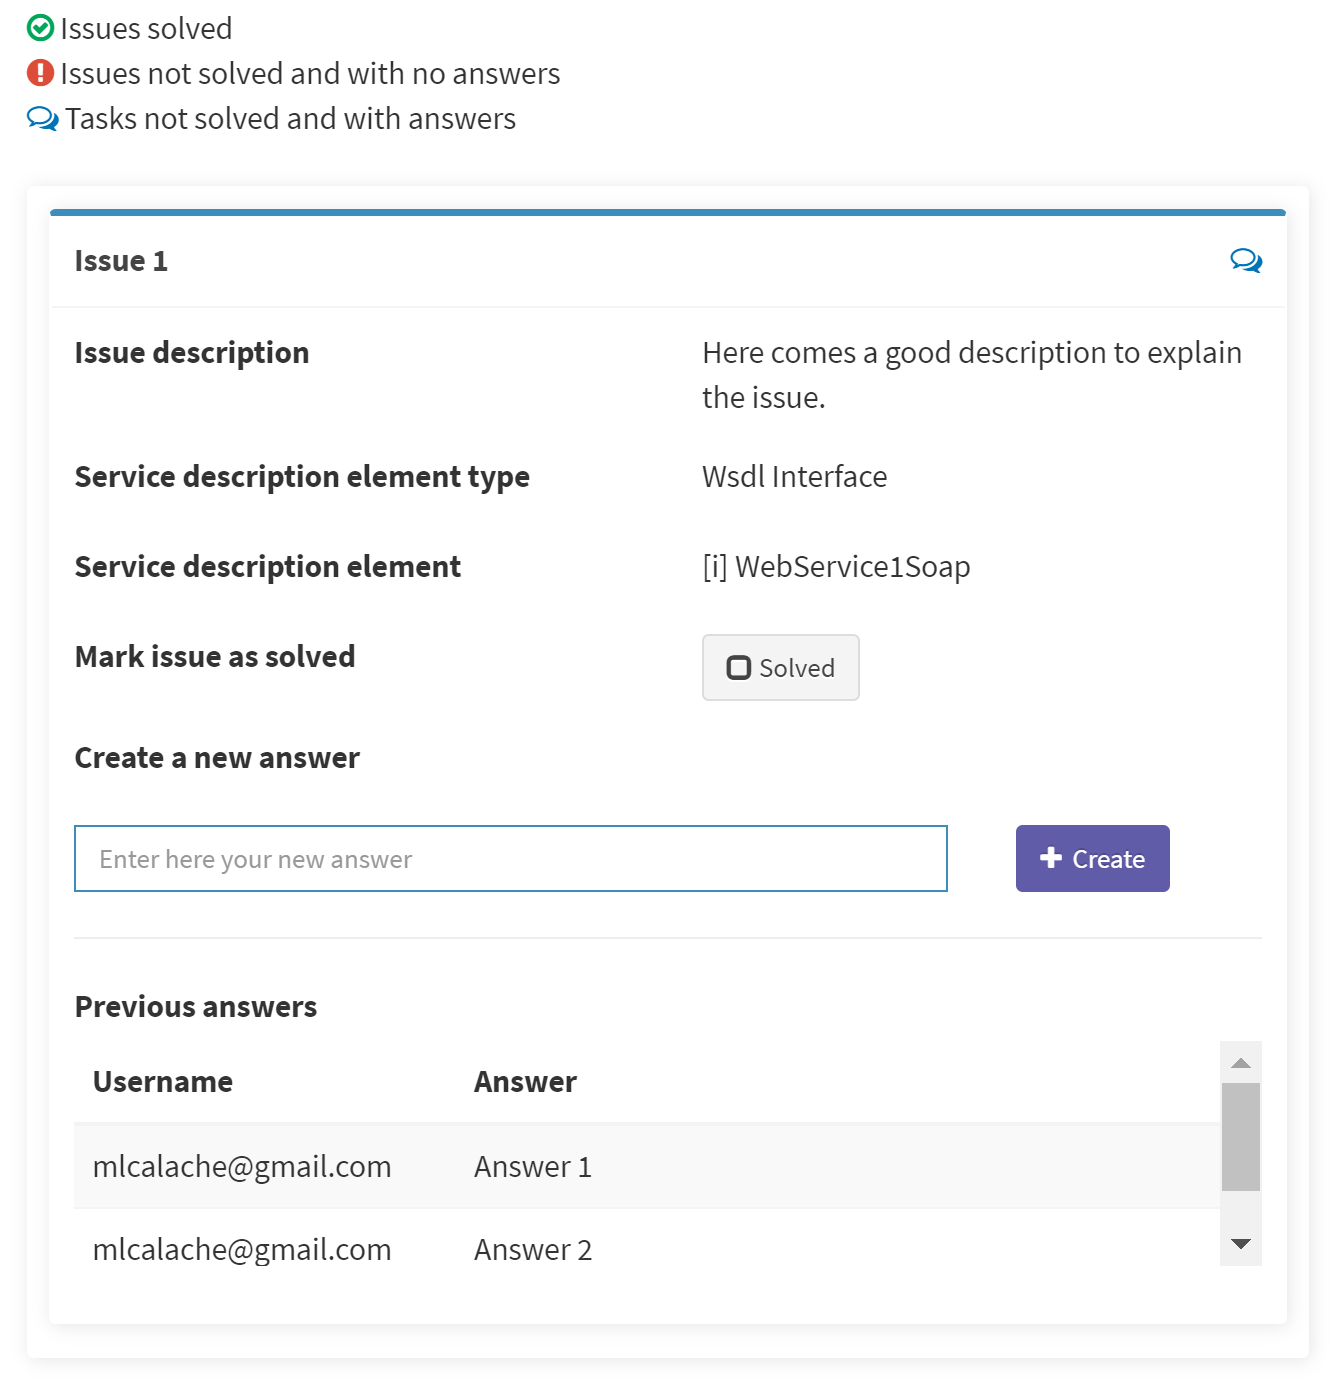
\includegraphics[scale=0.25]{4-grasews/imagens/grasews-lista-issues.png}
    %}
    \centering
    \caption[Interface gráfica para a lista de questões]{\textbf{Interface gráfica para a lista de questões.}}
    \label{fig:grasews-lista-issues}
\end{figure}

%Caso o usuário que criou a questão julgar que esta foi já propriamente respondida, este usuário pode marcar a questão como resolvida. Caso um elemento WSDL/XSD tenha todas as suas questões resolvidas, a representação visual deste elemento no grafo é automaticamente atualizada. Com isso, o elemento WSDL/XSD deixará de ser representado na cor amarela, conforme a notação visual proposta por este trabalho.

Quando um elemento WSDL/XSD possui uma questão não resolvida, o grafo WSDL de Grasews representa visualmente este elemento na cor amarela, substituindo, portanto, a cor original deste elemento. Caso o elemento WSDL/XSD não possua mais questões relacionadas, este elemento é representado em sua cor original conforme a notação visual proposta por este trabalho.

A \figurename~\ref{fig:grasews-anotacao-semantica-compartilhada-com-questoes} ilustra diferentes notações visuais envolvendo a anotação semântica de forma colaborativa e auxiliada por questões. A especificação WSDL exemplificada pela  \figurename~\ref{fig:grasews-anotacao-semantica-compartilhada-com-questoes} está compartilhada entre dois usuários: \texttt{Usuário A} e \texttt{Usuário B}. A \figurename~\ref{fig:grasews-anotacao-semantica-compartilhada-com-questoes}a ilustra a interface \texttt{MyWebService} para ambos os usuários em seu estado inicial, sem \textit{Model Reference} e sem questão. A \figurename~\ref{fig:grasews-anotacao-semantica-compartilhada-com-questoes}b ilustra a interface \texttt{MyWebService} com uma questão adicionada pelo \texttt{Usuário A}. O \texttt{Usuário B} responde esta questão, que auxiliou o \texttt{Usuário A} a anotar este elemento. A \figurename~\ref{fig:grasews-anotacao-semantica-compartilhada-com-questoes}c ilustra a interface \texttt{MyWebService} anotada e ainda com a questão. Finalmente, após ter realizada a anotação semântica, o \texttt{Usuário A} marca a sua questão como resolvida. A \figurename~\ref{fig:grasews-anotacao-semantica-compartilhada-com-questoes}d ilustra, portanto, a notação visual deste elemento, agora com \textit{Model Reference} e sem questão. 

\begin{figure}[h]
    %\resizebox{\textwidth}{!}{
        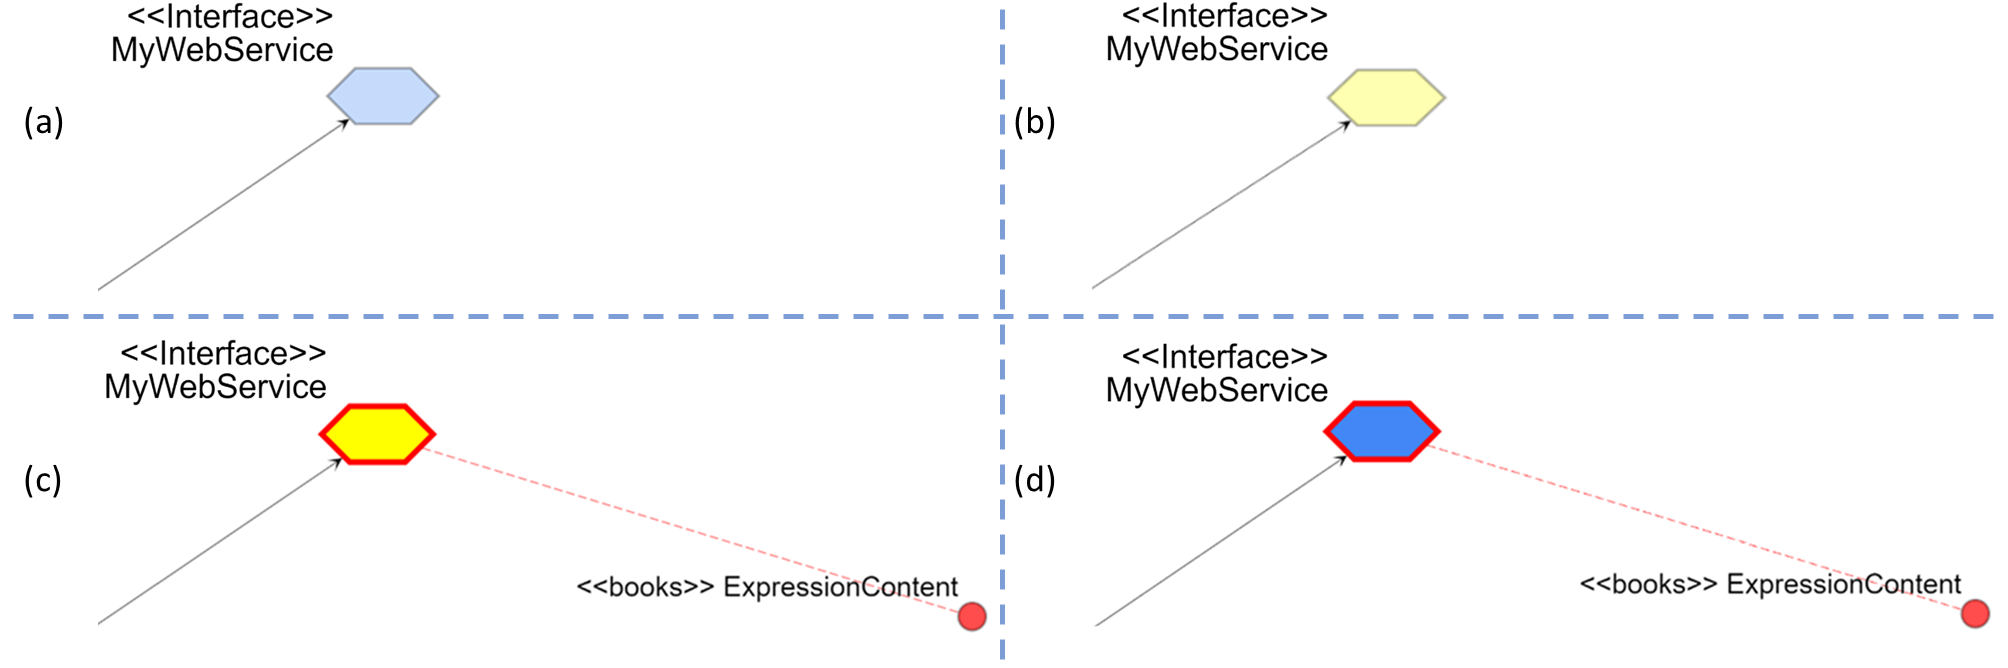
\includegraphics[scale=0.3]{4-grasews/imagens/grasews-anotacao-semantica-compartilhada-com-questoes.png}
    %}
    \centering
    \caption[Uso de questões para a anotação semântica de forma compartilhada]{\textbf{Uso de questões para a anotação semântica de forma compartilhada.} (a) Estado inicial da interface WSDL. (b) Interface WSDL com questão associada. (c) Interface WSDL com \textit{Model Reference} e com questão associada. (d) Interface WSDL com \textit{Model Reference}.}
    \label{fig:grasews-anotacao-semantica-compartilhada-com-questoes}
\end{figure}

Uma tarefa representa uma lista do trabalho necessário a ser realizado para concluir o processo de anotação semântica. A definição de uma ou mais tarefas pode contribuir para a coordenação do processo e anotação semântica entre múltiplos usuários envolvidos. Quando uma tarefa é concluída, esta tarefa pode ser marcada desta forma pelo usuário que a criou. Assim, os usuários mantém o controle das tarefas ainda pendentes de serem feitas.

Uma tarefa não é direcionada a um usuário específico, i.e., qualquer usuário envolvido na edição colaborativa é capaz de visualizar as tarefas para uma especificação WSDL. Além de visualizar a lista de tarefas, os usuários podem adicionar comentários, podendo contribuir para a finalização de uma tarefa. É possível ter múltiplos comentários de múltiplos usuários. A \figurename~\ref{fig:grasews-lista-tasks} ilustra a interface gráfica de Grasews para a listagem de tarefas. Por meio desta interface gráfica, um usuário pode adicionar comentários às tarefas e marcá-las como concluídas.

\begin{figure}[h]
    %\resizebox{\textwidth}{!}{
        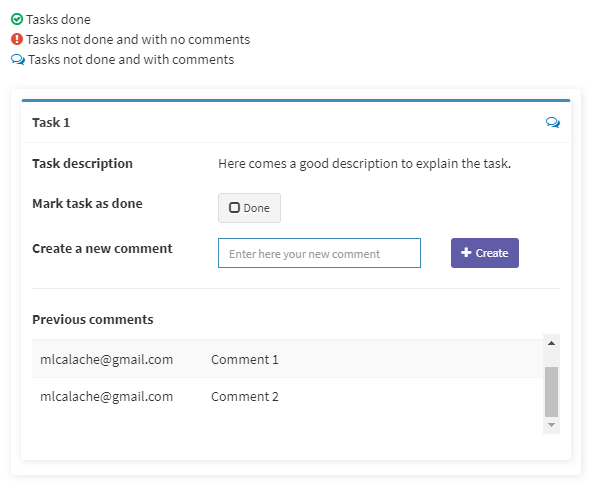
\includegraphics[scale=0.6]{4-grasews/imagens/grasews-lista-tasks.png}
    %}
    \centering
    \caption[Interface gráfica para a lista de tarefas]{\textbf{Interface gráfica para a lista de tarefas.}}
    \label{fig:grasews-lista-tasks}
\end{figure}